\section{Chapter 24: The Difference-in-Differences Saga}
\subsection{Panel data and two-way fixed effects}
\sourcepages{Chapter24-25.pdf, pp. 2 and 1; p. 1 continues the assumptions at the bottom of p. 2.}
\textbf{Panel data:} repeatedly observing the same unit over time. The example compares units across time and across regions. The drawing has an early-treated group (June 1), a later-treated group (July 15), and a control group; a faint extra trajectory is labelled \emph{TWFE prediction / counterfactual}.
\begin{center}
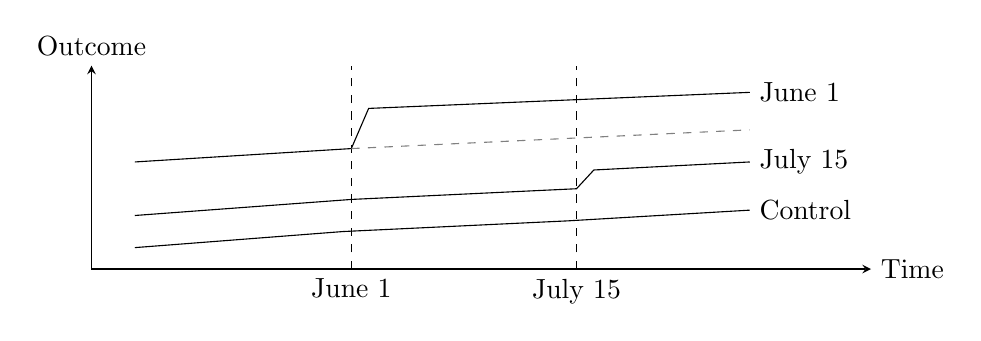
\begin{tikzpicture}[x=1.1cm,y=0.68cm,>=stealth]
\draw[->] (0,0)--(9,0) node[right]{Time};
\draw[->] (0,0)--(0,3.8) node[above]{Outcome};
\draw[dashed] (3,0)--(3,3.8);
\draw[dashed] (5.6,0)--(5.6,3.8);
\node[below] at (3,0){June 1}; \node[below] at (5.6,0){July 15};
\draw (0.5,.4)--(2.9,.7)--(5.5,.9)--(7.6,1.1) node[right]{Control};
\draw (0.5,1)--(3,1.3)--(5.6,1.5)--(5.8,1.85)--(7.6,2) node[right]{July 15};
\draw (0.5,2)--(3,2.25)--(3.2,3)--(7.6,3.3) node[right]{June 1};
\draw[gray,dashed] (3,2.25)--(7.6,2.6);
\end{tikzpicture}

{\small Schematic reconstruction of the handwritten trajectories; no numerical data are implied.}
\end{center}
Group units by their intervention date \(g\) (three groups in the example). The target written in the notes is
\[
\operatorname{ATT}=E[Y_1\mid t>g]-E[Y_0\mid t>g].
\]
The model is
\[
\mathrm{Install}_{it}=\tau D_{it}+\gamma_i+\theta_t+e_{it}.
\]
Here \(i\) denotes a unit, \(t\) time, and \(e_{it}\) noise; \(\gamma_i\) is associated with \(i\) and \(\theta_t\) with \(t\). Estimating this by OLS gives the \textbf{two-way fixed effects (TWFE)} model.

\paragraph{Author's annotations.}
At the same time, control for all characteristics. The red note connects TWFE and DiD: with two groups and two periods, this becomes DiD.
The notes write the mathematically equivalent residualized regression as
\[
\widetilde{\mathrm{Install}}_{it}=\tau\widetilde D_{it}+e_{it},
\]
with the following demeaning expressions:
\begin{align*}
\widetilde{\mathrm{Install}}_{it}
 &=\mathrm{Install}_{it}
 -\underbrace{\frac1T\sum_{t=0}^{T}\mathrm{Install}_{it}}_{\text{time average}}
 -\underbrace{\frac1N\sum_{i=0}^{N}\mathrm{Install}_{it}}_{\text{unit average}},\\
\widetilde D_{it}
 &=D_{it}-\frac1T\sum_{t=0}^{T}D_{it}-\frac1N\sum_{i=0}^{N}D_{it}.
\end{align*}
\textit{Translator's note:} These reproduce the scan, including summation endpoints. The usual double-demeaning expression also adds back the overall mean. This is a notation issue in the manuscript, not a change made in the translation.

\subsection{Death: Failures over Effect Heterogeneity}
TWFE often has bias when effects are heterogeneous. The fixed-effects model without time effects is written as
\[
y_{it}=\tau D_{it}+\gamma_i+e_{it}.
\]
The assumptions listed in the notebook are:
\begin{enumerate}
\item \textbf{Functional form:} no heterogeneous effect over time (constant effects); linearity in the covariates; additive fixed effects.
\item \textbf{Strict exogeneity:} parallel trends; no anticipation; no unobserved time-varying confounders; past treatment does not affect the current outcome (no carryover); past outcomes do not affect current treatment (no feedback).
\end{enumerate}
The second item is the left-page continuation connected by the arrow at the foot of the main page.

\sourcepages{Chapter24-25.pdf, p. 3.}
Continuing the previous point: suppose the treatment effect is heterogeneous over time, and the treatment response is gradual (from \(0.1,0.2,\ldots\), increasing from day to day). The ATT estimated by TWFE is then biased.
The drawing labels the early-treated group \(1\), the late-treated group \(2\), and the never-treated group \(3\). Decomposing TWFE into several \(2\times2\) DiDs gives:
\[
1-3:\ \checkmark,\quad
2-3:\ \checkmark,\quad
1-2:\ \checkmark,\quad
2-1:\ \text{??}
\]
The second member of each comparison is the control. \textbf{Author's intuition:} if the early-treated group \(1\) is used as the control, the model thinks that the untreated outcome \(Y_0\) would have risen in parallel with that group's earlier trajectory. The purple curve in the drawing is this estimated \(Y_0\), not the observed late-group outcome.

The notebook attributes this shorthand to Goodman-Bacon (2019):
\[
\operatorname*{plim}_{n\to\infty}\widehat\tau^{\mathrm{TWFE}}
 =\mathrm{VWATT}-\Delta\mathrm{ATT}.
\]
The purple annotation interprets the bias term as the extent to which ATT changes over time. If the effect increases over time, as in the drawing, the bias is downward; in the opposite case it is upward. \textbf{Author's warning:} with negative effects that decay over time, even the estimated sign can be wrong.
\textit{Translator's note:} The limit subscript is indistinct; \(n\to\infty\) renders the apparent probability-limit notation. VWATT is retained as written.

\subsection{Event-study design}
Rewrite TWFE using event-time indicators. The lead/lag expansion in the notes is rendered below with its uncertain final separator made explicit:
\begin{align*}
Y_{it}={}&\tau^{-K}D_{ik}^{<-K}
 +\sum_{k=-K}^{-2}\tau^{\mathrm{lead}}D_{it}^{k}
 +\sum_{k=0}^{L}\gamma_k^{\mathrm{lag}}D_{it}^{k}\\
 &+\gamma_k^{L+}D_{it}^{>L}+\gamma_i+e_{it},\\
D_{it}^{k}={}&\mathbf1\{t-\mathrm{Cohort}_i=k\}.
\end{align*}
The indicator is \(1\) if the relative period equals \(k\), and \(0\) otherwise. \textbf{Author's annotation:} add a variable measuring how far a unit is from its treatment start date. This is labelled a \emph{partial improvement}.
\textit{Translator's note:} The early-tail subscript looks like \(ik\); the lower lead-sum bound is faint; the sign before \(\gamma_i\) is missing or unclear. The displayed equation uses \(k=-K\) and a separating plus, but retains the manuscript's coefficient labels. No time fixed effect has been added.

\subsection{Enlightenment: A Flexible Functional Form}
\sourcepages{Chapter24-25.pdf, p. 4.}
A new model gives every individual a treatment effect at every time:
\[
\mathrm{Installs}_{it}
 =\sum_{i=0}^{N}\sum_{t=0}^{T}\tau_{it}D_{it}+\gamma_i+\theta_t+e_{it}.
\]
There are too many parameters. Instead, assign an effect to each group \(g\) at each time:
\[
\mathrm{Installs}_{it}
 =\sum_{g=0}^{G}\sum_{t=0}^{T}\tau_{gt}D_{it}+\gamma_i+\theta_t+e_{it}.
\]
This is marked as a better version. Reduce the parameters further by removing pre-treatment coefficients and the control-group coefficients:
\[
\mathrm{Installs}_{it}
 =\sum_{g=q}^{G}\sum_{t\geq g}^{T}\tau_{gt}D_{it}+\gamma_i+\theta_t+e_{it}.
\]
Cohorts with \(g<q\) are defined as controls. \textbf{Author's annotation:} one needs to create cohort dummy variables manually, such as \((0,1),(1,0),\ldots\).
\textit{Translator's note:} These sums reproduce the notebook's compact notation. Cohort-by-time indicators are not fully written out; the note about dummy variables explains the intended expansion.
Remaining limitations:
\begin{enumerate}
\item Treatment effects can change as time passes; this was not considered before.
\item DiD and TWFE must satisfy the parallel-trends assumption. The restriction is very strong.
\end{enumerate}

\section{Chapter 25: Synthetic Difference-in-Differences}
\subsection{Representing panel data}
\sourcepages{Chapter24-25.pdf, p. 5.}
There are multiple units over multiple periods, with treated and untreated observations mixed together. In \(D\), \textbf{rows are times and columns are units}:
\[
D=\begin{pmatrix}
0&0&0&\cdots&0&0\\
0&0&0&\cdots&0&0\\
\vdots&\vdots&\vdots&&\vdots&\vdots\\
0&0&0&\cdots&1&1\\
0&0&0&\cdots&1&1
\end{pmatrix}.
\]
The final columns identify the treated units. The note calls this \emph{one-time treatment} and stars the design requirement: once a unit is treated, it does not return to an untreated state.

\paragraph{Representation 1: synthetic control.}
Collapse the display into four blocks:
\[
D=\begin{pmatrix}0&0\\0&1\end{pmatrix},\qquad
Y=\begin{pmatrix}
Y_{\mathrm{pre,co}}&Y_{\mathrm{pre,tr}}\\
Y_{\mathrm{post,co}}&Y_{\mathrm{post,tr}}
\end{pmatrix}.
\]
Here pre means before treatment, post after treatment, co control group, and tr treatment group.
\paragraph{Representation 2: DiD.}
Use a long table with columns for unit, time, outcome, whether the unit belongs to the treatment group, and whether it has already been treated.
The observed outcomes are
\[
Y=\begin{pmatrix}
Y(0)_{\mathrm{pre,co}}&Y(0)_{\mathrm{pre,tr}}\\
Y(0)_{\mathrm{post,co}}&Y(1)_{\mathrm{post,tr}}
\end{pmatrix},
\]
and
\[
\operatorname{ATT}=Y(1)_{\mathrm{post,tr}}
-\underbrace{Y(0)_{\mathrm{post,tr}}}_{\text{missing}}.
\]

\subsection{Revisiting DiD and synthetic controls}
\sourcepages{Chapter24-25.pdf, pp. 6 and 7; p. 7 supplies the two comparison sketches.}
The DiD regression is
\[
Y_{it}=\beta_0+\beta_1\mathrm{Post}_t+\beta_2\mathrm{Treated}_i
+\beta_3\mathrm{Treated}_i\mathrm{Post}_t+e_{it}.
\]
Its assumption is
\[
E[Y(0)_{\mathrm{post,co}}-Y(0)_{\mathrm{pre,co}}]
=E[Y(0)_{\mathrm{post,tr}}-Y(0)_{\mathrm{pre,tr}}].
\]
That is, in the absence of treatment the control and treatment groups have the same trend.

Rewrite the estimator in a form comparable to SDID:
\[
\widehat\tau^{\mathrm{did}}
=\operatorname*{argmin}_{\mu,\alpha,\beta,\tau}
\left\{\sum_{i=1}^{N}\sum_{t=1}^{T}
[Y_{it}-(\mu+\alpha_i+\beta_t+\tau D_{it})]^2\right\}.
\]
The notes connect this to demeaning:
\begin{align*}
\widetilde Y_{it}
&=Y_{it}-\overline Y_i-\overline Y_t
=Y_{it}-T^{-1}\sum_{t=0}^{T}Y_{it}-N^{-1}\sum_{i=0}^{N}Y_{it},\\
\widetilde D_{it}
&=D_{it}-\overline D_i-\overline D_t
=D_{it}-T^{-1}\sum_{t=0}^{T}D_{it}-N^{-1}\sum_{i=0}^{N}D_{it}.
\end{align*}
This looks like synthetic controls, but lacks the weights.
\textit{Translator's note:} The \(\arg\min\) formulas use \(\widehat\tau\) as shorthand for the treatment-coefficient component of the joint minimizer. The missing grand means are preserved from the scan.

For synthetic control, estimate weights using pre-treatment outcomes:
\[
\widehat w^{\mathrm{sc}}
=\operatorname*{argmin}_{w}
\|\overline y_{\mathrm{pre,tr}}-Y_{\mathrm{pre,co}}w_{\mathrm{co}}\|_2^2,
\qquad \sum_iw_i=1,\quad w_i>0\quad\forall i.
\]
Here \(Y_{\mathrm{pre,co}}\) is a \(T_{\mathrm{pre}}\times N_{\mathrm{co}}\) outcome matrix: columns are units and rows are time periods. The vector \(w_{\mathrm{co}}\) has size \(N_{\mathrm{co}}\times1\). Each entry of \(\overline y_{\mathrm{pre,tr}}\) is the average of the treated units at a pre-treatment time.

\paragraph{Author's annotations.}
Fit a synthetic control to the treated group; this is similar to linear regression. After treatment, use the control outcomes and the fitted weights:
\[
y_{\mathrm{sc}}=Y_{\mathrm{co}}\widehat w^{\mathrm{sc}}.
\]
This gives a good estimate of \(Y(0)_{\mathrm{post,tr}}\). Thus
\[
\widehat\tau=\overline y_{\mathrm{post,tr}}-\overline y_{\mathrm{post,sc}}.
\]
Rewrite it as
\[
\widehat\tau^{\mathrm{sc}}
=\operatorname*{argmin}_{\beta,\tau}
\left\{\sum_{i=1}^{N}\sum_{t=1}^{T}
(Y_{it}-\beta_t-\tau D_{it})^2\widehat w_i^{\mathrm{sc}}\right\}.
\]
The pre-treatment fitting step provides control-group weights; each treated unit has weight \(1/N_{\mathrm{tr}}\). Purple annotations emphasize: \textbf{no overall intercept \(\mu\), and no unit fixed effects \(\alpha_i\).}

\paragraph{Left-page visual intuition (p. 7).}
The DiD sketch shifts a trajectory into a parallel comparison; the handwritten comment says this amplifies the effect in the illustrated case. In the SC sketch, pre-treatment data generate weights and hence a synthetic untreated treatment group. Use the same weights to compute post-treatment outcomes, and estimate the effect from the difference between the two post-treatment values. The curves closely track before treatment, then separate.
\begin{center}
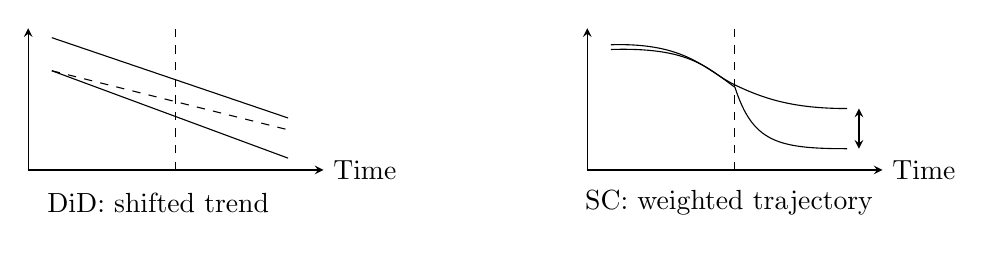
\begin{tikzpicture}[x=0.75cm,y=0.6cm,>=stealth]
\draw[->] (0,0)--(5,0) node[right]{Time};
\draw[->] (0,0)--(0,3);
\draw[dashed] (2.5,0)--(2.5,3);
\draw (0.4,2.8)--(4.4,1.1);
\draw (0.4,2.1)--(4.4,0.25);
\draw[dashed] (0.4,2.1)--(4.4,0.85);
\node at (2.2,-0.7){DiD: shifted trend};
\begin{scope}[xshift=7.1cm]
\draw[->] (0,0)--(5,0) node[right]{Time};
\draw[->] (0,0)--(0,3);
\draw[dashed] (2.5,0)--(2.5,3);
\draw (0.4,2.65) .. controls (1.7,2.7) and (2,2.1) .. (2.5,1.8)
.. controls (3,1.5) and (3.5,1.3) .. (4.4,1.3);
\draw (0.4,2.55) .. controls (1.7,2.6) and (2,2.2) .. (2.5,1.75)
.. controls (2.8,0.6) and (3.2,.45) .. (4.4,.45);
\draw[<->] (4.6,.45)--(4.6,1.3);
\node at (2.4,-0.7){SC: weighted trajectory};
\end{scope}
\end{tikzpicture}

{\small Schematic reconstructions of the author's sketches.}
\end{center}


\subsection{Combining the two: synthetic DiD}
\sourcepages{Chapter24-25.pdf, pp. 8 and 10 (upper and middle portions).}
The starred heading combines the synthetic-control weighted criterion and the DiD fixed-effects criterion:
\[
\widehat\tau^{\mathrm{sdid}}
=\operatorname*{argmin}_{\mu,\alpha,\beta,\tau}
\left\{\sum_{i=1}^{N}\sum_{t=1}^{T}
[Y_{it}-(\mu+\alpha_i+\beta_t+\tau D_{it})]^2
\underbrace{\widehat w_i^{\mathrm{sdid}}}_{\text{unit weight}}
\underbrace{\widehat\lambda_t^{\mathrm{sdid}}}_{\text{time weight}}\right\}.
\]
\paragraph{Time weights.}
Fit the average post-treatment outcome of the controls from their pre-treatment outcomes:
\[
\widehat\lambda^{\mathrm{sdid}}
=\operatorname*{argmin}_{\lambda}
\|\overline y_{\mathrm{post,co}}
-(\lambda_{\mathrm{pre}}Y_{\mathrm{pre,co}}+\lambda_0)\|_2^2,
\qquad \sum_t\lambda_t=1,\quad\lambda_t>0.
\]
\begin{itemize}
\item \(Y_{\mathrm{pre,co}}\) is \(T_{\mathrm{pre}}\times N_{\mathrm{co}}\); rows are times and columns are units.
\item \(\overline y_{\mathrm{post,co}}\) is a \(1\times N_{\mathrm{co}}\) row vector. Each entry is a control unit's time-averaged outcome after treatment.
\item \(\lambda_{\mathrm{pre}}\) is a \(1\times T_{\mathrm{pre}}\) row vector, with a weight for every pre-treatment period. \(\lambda\) is a time weight.
\end{itemize}
The arrows at the bottom of p. 8 show multiplication along the time dimension: prepend a row of ones to the matrix for the intercept, and fit \(\overline y_{\mathrm{post,co}}\) from the weighted pre-treatment rows to obtain \(\lambda_t\).
\textit{Translator's note:} The constraint looks like \(\lambda_t=1\) without a visible summation sign; the displayed sum-to-one reading follows the adjacent weighting construction. Several explanatory lines at the bottom are crossed out and replaced by this matrix sketch.

\paragraph{Unit weights.}
The small diagram at the top of p. 10 connects control/pre to control/post by \(\lambda\), and control/pre to treated/pre by \(w\), giving the corresponding treated/post comparison.
\begin{align*}
\widehat w^{\mathrm{sdid}}
=\operatorname*{argmin}_{w}\ \big\{
&\|\overline y_{\mathrm{pre,tr}}
-(Y_{\mathrm{pre,co}}w_{\mathrm{co}}+w_0)\|_2^2\\
&+\zeta^2T_{\mathrm{pre}}\|w_{\mathrm{co}}\|_2^2\big\},
\qquad \sum_iw_i=1,\quad w_i>0,\\
\zeta&=(N_{\mathrm{tr}}T_{\mathrm{post}})^{1/4}
\widehat\sigma(\Delta_{it}),\\
\Delta_{it}&=Y_{it}-Y_{i,t-1}.
\end{align*}
Here \(\Delta_{it}\) is the first difference and \(\widehat\sigma(\Delta_{it})\) its standard deviation.

\paragraph{Author's annotations.}
The \(L_2\) penalty makes the nonzero weights more widely distributed. Compared with the previous SC, this version (1) has an intercept, and (2) uses an \(L_2\) penalty. The implementation instruction says to add a row of ones \emph{before \(\overline y_{\mathrm{pre,tr}}\)} as an intercept and perform the regression.
\textit{Translator's note:} This instruction is reproduced from the scan; the displayed model places the intercept in the predictors. The scan again abbreviates the constraint as \(w_i=1\); it is read here as sum-to-one, consistently with p. 6.

For the treated units and post-treatment times, use uniform weights \(1/N_{\mathrm{tr}}\) and \(1/T_{\mathrm{post}}\), respectively. \textbf{Author's intuition:} compared with SC, SDID pays attention only to data that are close to the expected treatment effect.

\subsection{Time-effect heterogeneity and staggered adoption}
\sourcepages{Chapter24-25.pdf, p. 10 (lower portion), then the p. 9 supplement.}
SDID makes it easy to estimate an effect for each period: simply run the procedure multiple times. In these handwritten matrices, subscripts on the zeros and ones identify the period.
\paragraph{Time-effect heterogeneity.}
The example is
\[
D=\begin{pmatrix}
0_1&0_1&0_1\\0_2&0_2&0_2\\0_3&0_3&1_3\\0_4&0_4&1_4
\end{pmatrix}.
\]
Applying SDID gives an average ATT over periods 3 and 4. To estimate these periods separately, use
\[
D_1=\begin{pmatrix}0_1&0_1&0_1\\0_2&0_2&0_2\\0_3&0_3&1_3\end{pmatrix},
\qquad
D_2=\begin{pmatrix}0_1&0_1&0_1\\0_2&0_2&0_2\\0_4&0_4&1_4\end{pmatrix}.
\]

\paragraph{Staggered adoption: left-page supplement.}
The notebook gives
\[
D=\begin{pmatrix}
0_1&0_1&0_1\\0_2&0_2&0_2\\0_3&0_3&1_3\\0_4&1_4&1_4
\end{pmatrix}.
\]
The first decomposition is
\[
D_1=\begin{pmatrix}0_1&0_1&0_1\\0_2&0_2&0_2\\0_4&1_4&1_4\end{pmatrix},
\qquad
D_2=\begin{pmatrix}0_1&0_1&0_1\\0_2&0_2&0_2\\0_3&0_3&1_3\end{pmatrix}.
\]
Weight the ATT from \(D_1\) by \(2/3\), and the ATT from \(D_2\) by \(1/3\). Alternatively, split by treated cohort:
\[
D_1=\begin{pmatrix}0_1&0_1\\0_2&0_2\\0_3&0_3\\0_4&1_4\end{pmatrix},
\qquad
D_2=\begin{pmatrix}0_1&0_1\\0_2&0_2\\0_3&1_3\\0_4&1_4\end{pmatrix}.
\]
The example underneath says: California, treated for 12 years; others, 8 years \(\times3\). The weighting calculation is
\[
\mathrm{ATT}_0\frac{12}{36}
+\left(\sum\mathrm{ATT}\right)\frac13\frac{3\times8}{36}.
\]
This preserves the author's treatment-duration weighting illustration.

\subsection{Placebo variance estimation}
\sourcepages{Chapter24-25.pdf, p. 11.}
Compared with SC, the notebook describes SDID as having lower error bars. SDID captures variation in outcomes over time and across units. This improves the SDID confidence interval and applies to a single treated unit.

For each control unit, pretend it received treatment and use SDID to estimate a placebo ATT. The notes write
\[
\widehat V_{\tau}^{\mathrm{placebo}}
=B^{-1}\sum_{b=1}^{B}
\left(\widehat\tau^{(b)}-\overline\tau^{(b)}\right)^2,
\qquad
\tau\in\widehat\tau^{\mathrm{sdid}}
\pm z_{\alpha/2}\sqrt{\widehat V_\tau}.
\]
The variance of these estimates is the SDID placebo variance; use it to construct the confidence interval. A parenthetical annotation says this is the same as SC.
\textit{Translator's note:} The superscript on the handwritten mean \(\overline\tau\) looks like \((b)\), and the normal critical value is written \(z_{\alpha/2}\). Both are retained. The intended placebo mean and quantile convention are not explicitly defined.

\section{Appendix: Debiasing and Prediction}
\sourcepages{Chapter24-25.pdf, p. 12.}
A heading note links the treatment of non-randomized data to \textbf{propensity scores} and \textbf{orthogonalization}.
\subsection{Debiasing with orthogonalization}
The purple annotation refers to Chapter 22. All features are contained in \(X\).
\begin{enumerate}
\item Take the first group of features and fit
\[
y_i=\theta_0+\theta_1X_{1i}+e_i.
\]
Obtain the residual
\[
y_i^*=y_i-(\widehat\theta_0+\widehat\theta_1X_{1i}).
\]
\item Use the first group of features to predict the second group:
\[
X_{2i}=\gamma_0+\gamma_1X_{1i}+e_i.
\]
Obtain the residual
\[
X_{2i}^*=X_{2i}-(\widehat\gamma_0+\widehat\gamma_1X_{1i}).
\]
\item Regress the outcome residual on the feature residual:
\[
y_i^*=\beta_0+\beta_2X_{2i}^*+e_i.
\]
\end{enumerate}

\subsection{Debiasing with propensity scores}
\sourcepages{Chapter24-25.pdf, p. 13.}
The purple annotation refers to Chapter 11. Weight each unit. For binary treatment,
\[
w_i=\frac{T}{P(T=1\mid X)}+\frac{1-T}{1-P(T=1\mid X)}.
\]
The next formula, labelled \emph{continuous} in the manuscript, is
\[
w_i=\sum_{k=0}^{K}\frac{\mathbf1\{T=k\}}{P(T=k\mid X)}.
\]
\textit{Translator's note:} The label is translated literally; the sum is a discrete, multiple-treatment-level expression.

\paragraph{Author's intuition.}
A unit with a high probability of treatment that nevertheless remains untreated essentially resembles a treated unit but is observed in the control group. It can be used to estimate \(Y_0\mid T=1\).
If propensity scores are unavailable, estimate them using the probability of receiving treatment as the target, with machine learning. A small numerical illustration mentions 20\%, 0.2, and receiving an email marked \(1\); the rest of that short line is unclear in the scan.

\paragraph{Weaknesses of propensity scores.}
\begin{enumerate}
\item When the propensity score is very small (\(e<0.05\)), the weight is too large: the observation effectively appears too many times and strongly influences the debiased dataset. The note mentions manual trimming. The purple annotation stresses \textbf{high variance}.
\item \textbf{Positivity or common support:} there must be enough overlap between the characteristics of treated and control units. If overlap is too limited, propensity-score adjustment does a poor job of removing the association.
\end{enumerate}
The red annotations add: manual intervention is not very advisable because it can introduce excessive subjective bias; do not extrapolate to population subsets where positivity does not hold.

\subsection{When prediction fails}
\sourcepages{Chapter24-25.pdf, p. 14.}
Prediction and causality. This is a heading-only page; no further notes are written beneath it.
